\documentclass[xcolor=table,9pt]{beamer}

\usetheme{Frankfurt}
\usecolortheme{crane}
\useinnertheme{circles}

\usepackage{color, colortbl}
\usepackage{amsmath}
\usepackage{graphicx}
\usepackage{float}
\usepackage{wrapfig}
\usepackage{multicol}
\usepackage{dcolumn,array}
\usepackage{booktabs}
\usepackage{geometry}
\usepackage{caption}
\usepackage{subcaption}
\usepackage{bbm}
\usepackage{bm}
\usepackage{natbib}
\usepackage{stackengine} 
\usepackage{multirow}

\definecolor{Gray}{gray}{0.8}

\stackMath


\begin{document}
\title{Sparse Bayesian Estimation of Regime-Switching Time Series }   
\author{Mario Giacomazzo } 
\date{6 March 2018} 

\frame{\titlepage} 



\frame{\frametitle{Background: Regime-Switching Time Series Models} 
\begin{itemize}
\item Purpose of Regime-Switching Time Series Models \\~\
	\begin{itemize}
	\item Regime-Dependent Dynamics
	\item Understand Volatility Changes
	\item Alternative Approach to Handling Nonstationary and Cyclical Phenomenon
	\item State-specific Forecasting
	\item Characterization and Classification
	\end{itemize}
\end{itemize}
}


\frame{\frametitle{Background: Regime-Switching Time Series Models} 
\begin{itemize}
\item Popularized for Economic and Financial Time Series \\~\
	\begin{itemize}
		\item Structural Breaks Between Periods of Recession and Expansion
		\item Unemployment Rates \citep{Montgomery1998,Koop1999,Deschamps2008}
		\item Gross Domestic Product \citep{Terasvirta1995}
		\item Stock Prices \citep{Li1995}
		\item Agricultural Prices \citep{Zeng2011}
		\item Extensive Study on 215 Macroeconomic Time Series \citep{Stock1998a} \\~\
	\end{itemize}
\item Applications in Other Areas \\~\
	\begin{itemize}
		 \item Epidemiology: Epidemic vs Nonepidemic States \citep{Lu2010}
 		\item Psychology: Mood Changes Under Bipolar Disorder \citep{Hamaker2010}
 		\item Traffic Management: Free Flow vs Congested States \citep{Kamarianakis2010}
 		\item Ecology: Temperature Changes Due to Climate Changes \citep{Battaglia2012}
	\end{itemize}
\end{itemize}
}


\frame{\frametitle{Background: Regime-Switching Time Series Models} 
\begin{itemize}
\item Two Main Types \\~\
\begin{itemize}
   \item Stochastic Regime Changes
   \begin{itemize}
   \item Markov Switching Autoregressive Model (MSAR) \citep{Hamilton1990}
   \item Transitions Determined by Latent States Following a Markov Process\\~\
   \end{itemize}
   \item Deterministic Regime Changes 
   \begin{itemize}
   \item Threshold Autoregressive Model (TAR) \citep{Tong1990,Tong2012}
   \item Smooth Transition Autoregressive Model (STAR) \citep{Terasvirta1992,Terasvirta2010}
   \item States are Determined by Evaluation of an Observable Variable at a Previously Known Time Point
   \end{itemize}
\end{itemize}
\end{itemize}
}

\frame{\frametitle{Background: Regime-Switching Time Series Models} 
Given autoregressive order $P$, let $\bm{x}_t'=[y_{t-1},y_{t-2},\cdots,y_{t-P}]$, $\bm{\alpha}'=[\alpha_1,\cdots,\alpha_P]$, and $\bm{\beta}'=[\beta_1,\cdots,\beta_P]$. Consider General 2-Regime Autoregressive Model:
$$y_t=(\mu_\alpha+\bm{x}'_t\bm{\alpha}+\epsilon_{\alpha,t})(1-G(z_{t}))+(\mu_\beta+\bm{x}'_{t}\bm{\beta}+\epsilon_{\beta,t})G(z_{t})$$

For heteroskedasticity, $\epsilon_{\alpha,t}\sim N(0,\sigma^2_\alpha)$ and  $\epsilon_{\beta,t}\sim N(0,\sigma^2_\beta)$. 

\begin{itemize}
\item Transition Function $G(z_t): \mathbb{R}\to\mathbbm{G}\subseteq[0,1]$
\begin{itemize}
\item TAR($P$): $G(z_t,\delta)=\mathbbm{1}_{\{z_t>\delta\}}(z_t)$
\item LSTAR($P$): $G(z_t,\gamma^*,\delta)=\{1+\exp[-(\gamma^*/s_Z)(z_t-\delta)]\}^{-1}$
\item ESTAR($P$): $G(z_t,\gamma^*,\delta)=1-\exp[-(\gamma^*/s_Z)(z_t-\delta)^2]$
\end{itemize}
\end{itemize}
Threshold $\delta$ and transition slope $\gamma=\gamma^*/s_Z$ are additional parameters which control  location and shape of the transition function.
}

\frame{\frametitle{Background: Regime-Switching Time Series Models} 
\begin{itemize}
\item Regime-switching Dependent on Transition Variable $z_t$
\begin{itemize}
	\item Low Regime: $z_t<\delta$
	\item High Regime: $z_t>\delta$
	\item Options for $z_t$ Given Delay Parameter $d$
	\begin{itemize}
		\item Exogenous Option: $z_t=r_{t-d}$
		\item Self-Exciting: $z_t=y_{t-d}$
		\item Time: $z_t=t$ \\~\
	\end{itemize}
\end{itemize}
\item As $\gamma \to \infty$, LSTAR and ESTAR Transition Functions Become Abrupt\\~\
\item Threshold $\delta\in [q_Z(.15),q_Z(0.85)]$ Where $q_Z(.)$ is the Empirical Quantile Function
\end{itemize}
}


\frame{\frametitle{Background: Regime-Switching Time Series Models} 
\begin{itemize}
\item Bayesian Estimation Methods\\~\
	\begin{itemize}
		\item TAR\citep{Geweke1993,Chen1995,Koop1999} and STAR\citep{Lubrano2000,Lopes2006,Livingston2017} \\~\
		\item Prior Distributions
		\begin{itemize}
			\item Normal Priors for $\mu_\alpha$, $\bm{\alpha}$,$\mu_\beta$, and $\bm{\beta}$
			\item Inverse Gamma Priors for $\sigma^2_\alpha$ and $\sigma^2_\beta$
			\item Gamma, Log-Normal, Truncated Normal, etc.  for $\gamma^*$
			\item  $\delta \sim Uniform[q_Z(0.15),q_Z(0.85)]$
			\item $p(d)=\frac{1}{d_{max}}$ for $d\in \{1,2,\cdots,d_{max}\}$
		\end{itemize}		
	\end{itemize}
\end{itemize}
}

\frame{\frametitle{Background: Regime-Switching Time Series Models} 
\begin{itemize}
\item Bayesian Estimation Methods (Cont.)\\~\
	\begin{itemize}
				\item Exploits the Conditional Linear Nature Given Parameters $\delta$ and/or $\gamma$ \\~\
		\item MCMC Sampling from Joint Posterior $f(\bm{\theta}|Data)$ where
		$$\bm{\theta}'=[\mu_\alpha,\bm{\alpha},\sigma^2_\alpha,\mu_\beta,\bm{\beta,\sigma^2_\beta},\gamma,\delta,d]$$
		\begin{itemize}
			\item Gibbs Sampler for Regime-specific Means, Coefficients, and Variances Using Full Conditional Distributions \citep{Gelfand1990}
			\item Metropolis-Hastings Approach for $\gamma$ and $\delta$ \citep{Metropolis1953, Hastings1970}
			\item Posterior Discrete Uniform Probabilities for $d \in \{1,2,\cdots,P\}$ Found Using Bayes' Rule
		\end{itemize}
	\end{itemize}
\end{itemize}
}

\frame{\frametitle{Background: Bayesian Model Selection} 
\begin{itemize}
\item Bayesian Inference for Model Order $P$\\~\
	\begin{itemize}
		\item Define $P$ as the Maximum Model Order Across Regimes \\~\
		\item Apply Bayesian Estimation for Many Choices of $P$ and Choose Based on Bayes' Factors \\~\
		\item Reversible jump Markov Chain Monte Carlo (RJMCMC) Used when $P$  in $\bm{\theta}$ 
		\begin{itemize}
			\item AR models \citep{Troughton1997,Vermaak2004}
			\item TAR or STAR models \citep{Campbell2004,Lopes2006}
			\item Why? $\dim(\bm{\Theta})$ depends on $P$\\~\
		\end{itemize}
		\item Required Assumptions for These Approach 
		\begin{itemize}
			\item Model Order $P$ is the Same in Both Regimes
			\item Given $P$, All Lagged Terms Less than $P$ are Significant\\~\
		\end{itemize}
		\item Problems Under Assumptions 
		\begin{itemize}
			\item Estimates Inflexible LSTAR Models Solely Determined by $P$
			\item Even if $P$ is Identified Correctly,  Overfitting  May Occur
		\end{itemize}
	\end{itemize}
\end{itemize}
}

\frame{\frametitle{Background: Transition} 
Consider the general matrix representation of the full linear model
\begin{equation*}
\def\sss{\scriptscriptstyle}
\setstackgap{L}{8pt}
\def\stacktype{L}
\stackunder{\bm{y}}{\sss T\times 1} =  \stackunder{\bm{X}}{\sss T\times P} \times 
\stackunder{\bm{\theta}}{\sss P\times 1} + \stackunder{\bm{\epsilon}}{\sss T\times 1}
\end{equation*}
Although we consider $P$ covariates, it is possible that $\bm{\theta}$ contains many $0$ entries. For high-dimensional scenarios (Large $P$), sparse estimation of $\bm{\theta}$ becomes important to combat overfitting and identify the underlying signal.\\~\

See \cite{Dellaportas2002,OHara2009,Polson2010} for an Overview of Bayesian Approaches to Finding the ``Best'' Model.
}

\frame{\frametitle{Background: Bayesian Variable Selection} 
\begin{itemize}
 	\item Binary Indicator Variables Used To Identify Covariate Inclusion.
           Each submodel $\bm{m} \in \mathcal{M}=\{0,1\}^P$ is a $P\times1$  vector of binary indicators. 
 	\begin{equation*}
		\bm{y}=  \bm{X}_m\bm{\theta}_m + \bm{\epsilon}
	\end{equation*}
	\item Exploring $\mathcal{M}$ is Time Consuming and Difficult. $2^P$ Possible Models
	\item Popular Prior: $$m_k \sim Bern(\pi_k)$$
	Choice of $\pi_k$ reflects prior beliefs on the true model complexity. Typically $\pi_k=\pi=0.5$
	\item Posterior MCMC Algorithms Incoporate $\bm{m}$. The Posterior Expectation $E[m_k|Data]$ Updates $\pi_k$
\end{itemize}
}

\frame{\frametitle{Background: Bayesian Variable Selection} 
\begin{itemize}
	\item Posterior Probability of Model $\bm{m}$
	$$P(\bm{m}|Data)=\frac{p(Data|\bm{m})p(\bm{m})}{\sum p(Data|\bm{m}_k)p(\bm{m}_k) }$$
	\item Bayes' Factor Comparing Two Candidates $\bm{m}_1$ and $\bm{m}_2$
	$$BF=\frac{p(Data|\bm{m}_1)}{p(Data|\bm{m}_2)}=\frac{p(\bm{m}_1|Data)p(\bm{m}_2)}{p(\bm{m}_2|Data)p(\bm{m}_1)}$$
	\item Inclusion Indicators Used in Spike and Slab Mixture Priors i.e. Stochastic Search Variable Selection \citep{George1993}
	$$p(\theta_k|m_k)=(1-m_k)N(0,\tau^2)+m_kN(0,g\tau^2)$$
	Typically, $\tau^2$ should be small and $g$ should be large.	
\end{itemize}
}


\frame{\frametitle{Background: Bayesian Shrinkage} 
\begin{itemize}
	\item Popular Regularization Methods
		$$\widehat{\bm{\theta}}=\underset{\bm{\theta}}{\textrm{argmin }} \frac{1}{T}(\bm{y}-\bm{X}\bm{\theta})'(\bm{y}-\bm{X}\bm{\theta}) + \lambda \times Penalty(\bm{\theta}) $$
	\begin{itemize}
		\item Ridge Regression: $Penalty(\bm{\theta})=||\bm{\theta}||_2^2$ \citep{Hoerl1970}
		\item Lasso Regression: $Penalty(\bm{\theta})=||\bm{\theta}||^1$ \citep{Tibshirani1996}
		\item Elastic Net: $Penalty(\bm{\theta})=\alpha||\bm{\theta}||_2^2+(1-\alpha)||\bm{\theta}||^1$ \citep{Zou2005}
	\end{itemize}
\end{itemize}
}

\frame{\frametitle{Background: Bayesian Shrinkage} 
\begin{itemize}
	\item Bayesian Regularization
	\begin{itemize}
		\item Priors Represented as Scale Mixtures of Normals with Continuous Mixing Densities
		\item Global-Local Hierarchical Representation
		$$\theta_k|\lambda^2_k,\lambda^2,\sigma^2 \sim N(0,\sigma^2\lambda^2\lambda^2_k)$$
		$$\lambda^2_k \sim p_{Local}(.) \textrm{ and  } \lambda^2 \sim p_{Global}(.)$$
		\item Different Priors for Local and Global Shrinkage Parameters Lead to:
		\begin{itemize}
			\item Different Concentration Around $0$
			\item Different Tail Behavior \\~\
		\end{itemize}
	\end{itemize}
	
	\item Optional Bayesian Shrinkage Methods
	\begin{itemize}
		\item Lasso \citep{Park2008}
		\item Horseshoe \citep{Carvalho2010,Makalic2016}
		\item Double-Pareto \citep{Armagan2013}
		\item Bridge \citep{Polson2014}
		\item Horsehoe+ \citep{Bhadra2016}
		\item Dirichlet-Laplace \citep{Bhattacharya2015}
	\end{itemize}
\end{itemize}
}




















%%%%%%%%%%%%%%%%%%%%%%%%%%%%%%%%%%%%%%%%%%%%%%
\frame{\frametitle{ Bayesian Shrinkage Estimation of LSTAR Models}
\begin{itemize}
\item Primary Goals \\~\
	\begin{itemize}
		\item Establish the Efficacy of Bayesian Shrinkage Estimation applied to LSTAR
		\item Modify Bayesian Shrinkage Priors to Handle Regime-specific Sparsity
		\item Allow for Composite Transition Variable to Be Estimated Using Dirichlet Prior
	\end{itemize}
\end{itemize}
}

\frame{\frametitle{Bayesian Shrinkage Estimation of LSTAR Models} 
\begin{itemize}
\item Bayesian Shrinkage Methods\\~\
\begin{itemize}
	\item Bayesian Lasso (BLASSO)
	\begin{equation*}
	\begin{split}
	\alpha_j|\sigma^2,\tau^2_{\alpha_j} \sim N(0,\sigma^2\tau^2_{\alpha_j}) \textrm{,  }  \tau^2_{\alpha_j}| \sim EXP(\lambda^2/2)\\ 
	 \beta_j|\sigma^2,\tau^2_{\beta_j}\sim N(0,\sigma^2\tau^2_{\beta_j}) \textrm{,  } \tau^2_{\beta_j}| \sim EXP(\lambda^2/2)
	\end{split}
\end{equation*}
	Hyperparameter $\lambda$ Controls Global Shrinkage Across Both Regimes. Following \cite{Park2008}, gamma hyperprior for $\lambda$ leads to inverse-Gaussian full conditional distribution.\\~\
	\item Regime-Specific Bayesian Lasso (RS-BLASSO) 
\begin{equation}
	 \tau^2_{\alpha_j}| \sim EXP(\lambda_1^2/2) \textrm{,  } \tau^2_{\beta_j}| \sim EXP(\lambda_2^2/2)
\end{equation}
Hyperparameters $\lambda_1$ and $\lambda_2$ control global shrinkage within low and high regimes, respectively.
\end{itemize}
\end{itemize}
}

\frame{\frametitle{ Bayesian Shrinkage Estimation of LSTAR Models} 
\begin{itemize}
\item Bayesian Shrinkage Methods (Cont.)\\~\
\begin{itemize}
	\item Variable Selection with Bayesian Lasso (VS-BLASSO) 
	Introducing latent binary variables $\zeta_j$ and $\eta_j$ for $j \in \{1,2,\cdots, p\}$, reparameterize $\alpha_j=\zeta_j\alpha_j^*$ and $\beta_j=\eta_j\beta_j^*$.
		\begin{equation*}
		\begin{split}
	 	\zeta_j \sim BERN(0.5) \textrm{,  } & \alpha_j^*|\sigma^2\sim DEXP\Big(0,\frac{\sigma^2}{\lambda}\Big) \\
	 	 \eta_j \sim BERN(0.5) \textrm{,  } & \beta_j^*|\sigma^2\sim DEXP\Big(0,\frac{\sigma^2}{\lambda}\Big)
		\end{split}
		\end{equation*}
	Method proposed by \cite{Lykou2011,Lykou2013}. Combines the subset selection approach of \cite{Kuo1998} with the Bayesian Lasso of  \cite{Park2008}.
\end{itemize}
\end{itemize}
}

\frame{\frametitle{ Bayesian Shrinkage Estimation of LSTAR Models} 
\begin{itemize}
\item Bayesian Shrinkage Methods (Cont.)\\~\
\begin{itemize}
	\item Bayesian Horseshoe (BHS)
	\begin{equation*}
	\begin{split}
	\alpha_j|\lambda_{\alpha_j} & \sim N(0,\lambda_{\alpha_j}) \textrm{,  }  \beta_j|\lambda_{\beta_j} \sim N(0,\lambda_{\beta_j}) \\
	  \lambda_{\alpha_j} & \sim C^+(0,\lambda) \textrm{,  } \lambda_{\beta_j} \sim C^+(0,\lambda) \\
	  \lambda|\sigma^2 & \sim C^+(0,\sigma)
	\end{split}
	\end{equation*}
	Although hyperparameter $\lambda$ provides global shrinkage, the additional  hyperparameters allow for finer shrinkage locally.
\end{itemize}
\end{itemize}
}

\frame{\frametitle{ Bayesian Shrinkage Estimation of LSTAR Models} 
\begin{itemize}
\item Estimation of Delay Parameter (Self-Exciting Case)\\~\
\begin{itemize}
\item Let $\bm{d}'_t=[y_{t-1},y_{t-2},\cdots,y_{t-d_{max}}]$ and $\bm{\phi}'_t=[\phi_{1},\phi_{2},\cdots,\phi_{d_{max}}]$. Reparameterize transition variable $z_t=\bm{\phi}'\bm{d}_t$. 

$$\bm{\phi}\sim Dir\bigg(\bigg[\frac{1}{d_{max}},\frac{1}{d_{max}},\cdots,\frac{1}{d_{max}}\bigg]'\bigg)$$

Now, $z_t$ is a weighted average of all considered transition variables. Because the weights are constrained to sum to $1$, the prior for $\delta$ does not require modification. \\~\

\item Advantages
\begin{itemize}
	\item Allows for a composite transition variable
	\item Estimates a more encompassing LSTAR model.
\end{itemize}
\end{itemize}
\end{itemize}
}


\frame{\frametitle{ Bayesian Shrinkage Estimation of LSTAR Models} 
\begin{itemize}
\item Initial Simulation Studies\\~\
\begin{itemize}
\item Evaluate Bayesian Shrinkage Methods on LSTAR 
\item Examine Effect of Increased Noise
\item Examine Performance  for Different Sparsity Patterns
\item Assume the Delay Parameter $d$ is known \textit{a priori}
\item All Replications are of Length $T=1000$
\item Assume Maximum Model Order $P=4$
\item Evaluation Based on  $RMSE(\theta)=\sqrt{\sum(\hat{\theta}-\theta)^2/N}$ Where $N$ Represents the Number of Replications
\end{itemize}
\end{itemize}
}

\frame{\frametitle{ Bayesian Shrinkage Estimation of LSTAR Models} 
\begin{itemize}
\item Computational Considerations \\~\
\begin{itemize}
	\item MCMC Sampling Using JAGS through R
	\item 3 Chains with Random Starting Values
	\item Burn-in=15,000, Thinning=10, Starting Sample=1,000
	\item Addtional Samples of 1000 Are Obtained Until...
	\begin{itemize}
		\item Potential Scale Reduction Factor (PSRF) Indicates Convergence ($<1.05$) for All Monitored Parameters
		\item Effective Sample Size (ESS) Is Large Enough ($>150$) for Alll Monitored Parameters
		\item Maximum of 20 Updates
	\end{itemize}
	\item Evaluate Methods and Calculate RMSE for Converged Replications
\end{itemize}
\end{itemize}
}

\frame{\frametitle{ Bayesian Shrinkage Estimation of LSTAR Models} 
\begin{itemize}
\item Simulation Study 1: Well-Behaved LSTAR
\begin{equation*}
	\begin{split}
		y_t&=(1.8y_{t-1}-1.06y_{t-2})[1-G(y_{t-2})]\\
		&+(0.02+0.9y_{t-1}-0.265y_{t-2})[G(y_{t-2})]+\epsilon_t\\
		& \textrm{where: } G(y_{t-2})=\bigg\{1+\exp\big[-100(y_{t-2}-0.02)\big]\bigg\}^{-1} \\
		&\textrm{ and }\epsilon_t \sim \textrm{i.i.d. }  N (0,0.02^2).\\
	\end{split}
\end{equation*}
Used in \cite{Lopes2006}
\end{itemize}
}

\frame{\frametitle{ Bayesian Shrinkage Estimation of LSTAR Models} 
\begin{itemize}
\item Simulation Study 1: Well-Behaved LSTAR (Cont.)
\begin{figure}[!h]
	\centering
      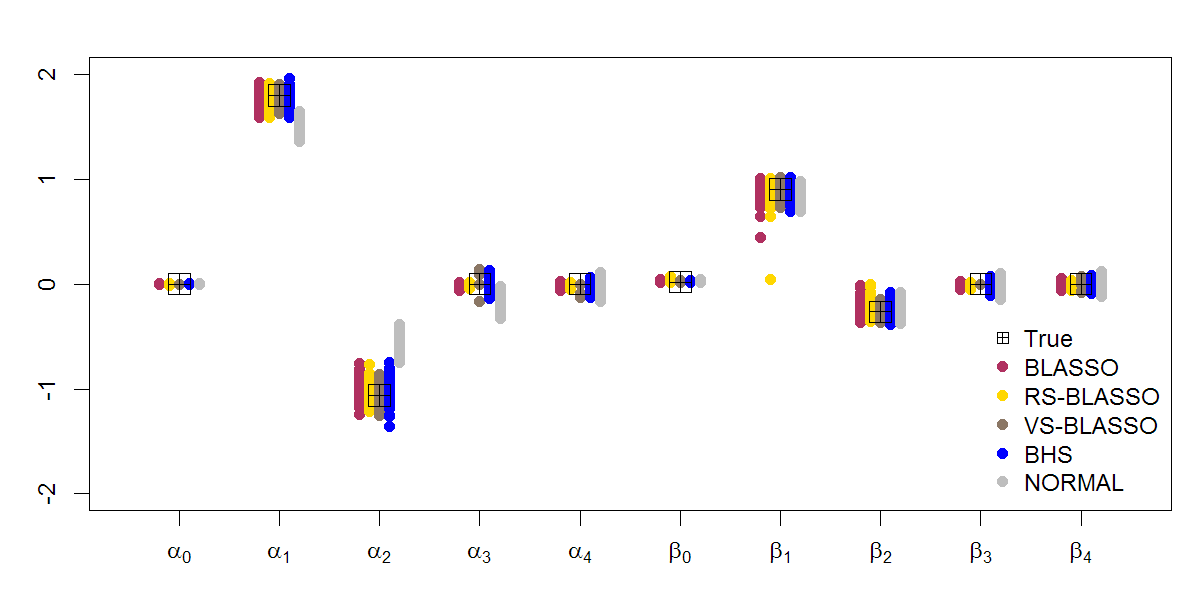
\includegraphics[scale=0.25]{blassovsbhs}
\end{figure}
\end{itemize}
}




\frame{\frametitle{ Bayesian Shrinkage Estimation of LSTAR Models} 
\begin{itemize}
\item Simulation Study 2: LSTAR With Gaps and Increased Noise 
\begin{equation*}
	\begin{split}
		y_t&=(-0.6y_{t-3})[1-G(y_{t-1})]\\
		 &+(0.02+0.75y_{t-3})[G(y_{t-1})]+\epsilon_t\\
		& \textrm{where: } G(y_{t-1})=\bigg\{1+\exp\big[-120(y_{t-1}-0.02)\big]\bigg\}^{-1} \\
		&\textrm{ and }\epsilon_t \sim \textrm{i.i.d. }  N (0,\sigma_k^2)\\
	\end{split}
\end{equation*}
We evaluate results for $\sigma_j=0.02j \textrm{ } \forall j\in \{1,2,\cdots,5\}$
\end{itemize}
}

\frame{\frametitle{ Bayesian Shrinkage Estimation of LSTAR Models} 
\begin{itemize}
\item Simulation Study 2: LSTAR With Gaps and Increased Noise (Cont.)
\begin{figure}[h]
      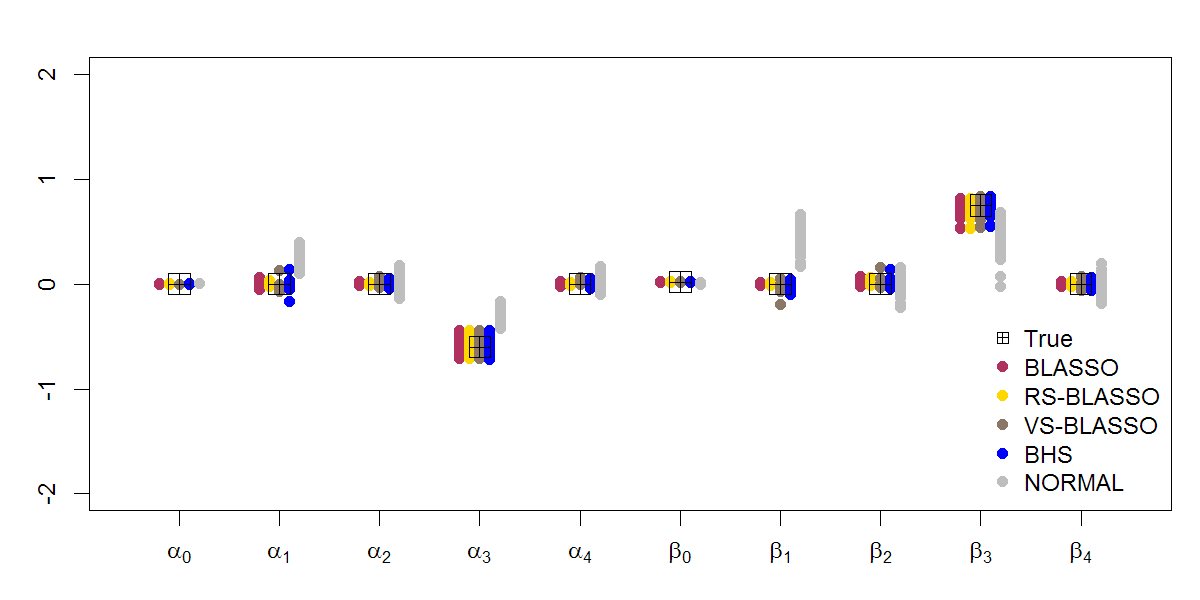
\includegraphics[scale=0.25]{blassovsbhs3}
\end{figure}
\end{itemize}
}

\frame{\frametitle{ Bayesian Shrinkage Estimation of LSTAR Models} 
\begin{itemize}
\item Simulation Study 2: LSTAR With Gaps and Increased Noise (Cont.)\\~\

Naturally, increases in $\sigma$ will cause increases in $s_y$. Recall the reparameterized transition slope $\gamma=\frac{\gamma^*}{s_y}$. For a fixed $\gamma=120$, increases in $\sigma$  indirectly increase $\gamma^*$. To ensure $\gamma^*$ stays constant, we target $\gamma^*\approx 4$ and simulate data with $\gamma_j \approx \frac{4}{s_y}$ for each proposed $\sigma_j=0.02j$.

\end{itemize}
}

\frame{\frametitle{ Bayesian Shrinkage Estimation of LSTAR Models} 
\begin{itemize}
\item Simulation Study 2: LSTAR With Gaps and Increased Noise (Cont.) \\~\
Table Gives RMSE for the Different Regime-Specific Coefficients.
\begin{table}[!h]
\scriptsize
  \centering
    \begin{tabular}{cc|cc|cc}
    \toprule
    Method & Parameter & \multicolumn{2}{c}{Fixed Transition Slope} & \multicolumn{2}{c}{Modified Transition Slope} \\
    \midrule
    \multicolumn{2}{r|}{Choice of $\sigma$} & 0.02 & 0.1 & 0.02 & 0.1 \\
    \multicolumn{2}{r|}{Choice of $\gamma$} & \multicolumn{2}{c|}{$120$} & 109.60 & 30.02 \\
    \midrule
    BLASSO & $\alpha_0$ & 0.0009 & 0.0032 & 0.001 & 0.0049 \\
    & $\alpha_1$ &  0.0068 & 0.013 & 0.0091 & 0.0258 \\
    & $\alpha_2$ & 0.0125 & 0.0102 & 0.0121 & 0.0136 \\
        \rowcolor{Gray}
    & $\alpha_3$ & 0.0479 & 0.0328 & 0.0501 &  0.0543 \\
    & $\alpha_4$ & 0.0119  & 0.0106 & 0.012 & 0.0099 \\
    & $\beta_0$ & 0.0019  & 0.0059 & 0.0019 & 0.0069 \\
    & $\beta_1$ & 0.006 & 0.0177 & 0.0069 & 0.0218 \\
    & $\beta_2$ & 0.0091  & 0.0151 & 0.0127 & 0.02 \\
        \rowcolor{Gray}
    & $\beta_3$ & 0.0494 &  0.0403 & 0.0579 & 0.0707 \\
    & $\beta_4$ & 0.008 &  0.0204 & 0.0093 & 0.0193 \\
    \midrule
    HS & $\alpha_0$ & 0.0011 &  0.0049 & 0.0011  & 0.0065 \\
    & $\alpha_1$ & 0.0054 & 0.0251 & 0.0063 & 0.0345 \\
    & $\alpha_2$ & 0.0075 & 0.0181 & 0.0074 & 0.0223 \\
    \rowcolor{Gray}
    & $\alpha_3$ & 0.0485 &  0.0334 & 0.0508 & 0.0568 \\
   & $\alpha_4$ & 0.0079 & 0.0174 & 0.008 & 0.02 \\
    & $\beta_0$ & 0.0018 &  0.0058 & 0.0018 & 0.0067 \\
    & $\beta_1$ & 0.004 & 0.0242 & 0.0039 & 0.0258 \\
    & $\beta_2$ & 0.0068 &  0.0237 & 0.0071 & 0.0261 \\
        \rowcolor{Gray}
   & $\beta_3$ & 0.0524  & 0.042 & 0.0608 &  0.0739 \\
    & $\beta_4$ & 0.0062 & 0.0258 & 0.0063 & 0.0259 \\
    \bottomrule
    \end{tabular}%
  \label{tab:changingsigma}%
\end{table}%
\end{itemize}
}

\frame{\frametitle{ Bayesian Shrinkage Estimation of LSTAR Models} 
\begin{itemize}
\item Simulation Study 3: LSTAR With Regime-Specific Sparsity
 \begin{equation*}
	\begin{split}
		\label{eq:sim3}
		y_t&=(-0.7y_{t-3})[1-G(y_{t-1})]\\
		&+(0.06+0.4y_{t-1}-0.35y_{t-2}+0.2y_{t-3})[G(y_{t-1})]+\epsilon_t\\
		& \textrm{where: } G(y_{t-1})=\bigg\{1+\exp\big[-120(y_{t-1}-0.03)\big]\bigg\}^{-1} \\
		&\textrm{ and }\epsilon_t \sim \textrm{i.i.d. }  N (0,0.02^2)\\
	\end{split}
\end{equation*}
\end{itemize}
}

\frame{\frametitle{ Bayesian Shrinkage Estimation of LSTAR Models} 
\begin{itemize}
\item Simulation Study 3: LSTAR With Regime-Specific Sparsity (Cont.)\\~\

Comparison of Posterior Distributions for Shrinkage Parameters from BLASSO ($\lambda$) and RS-BLASSO ($\lambda_1$ and $\lambda_2$)
\begin{figure}[!h]
	\centering
      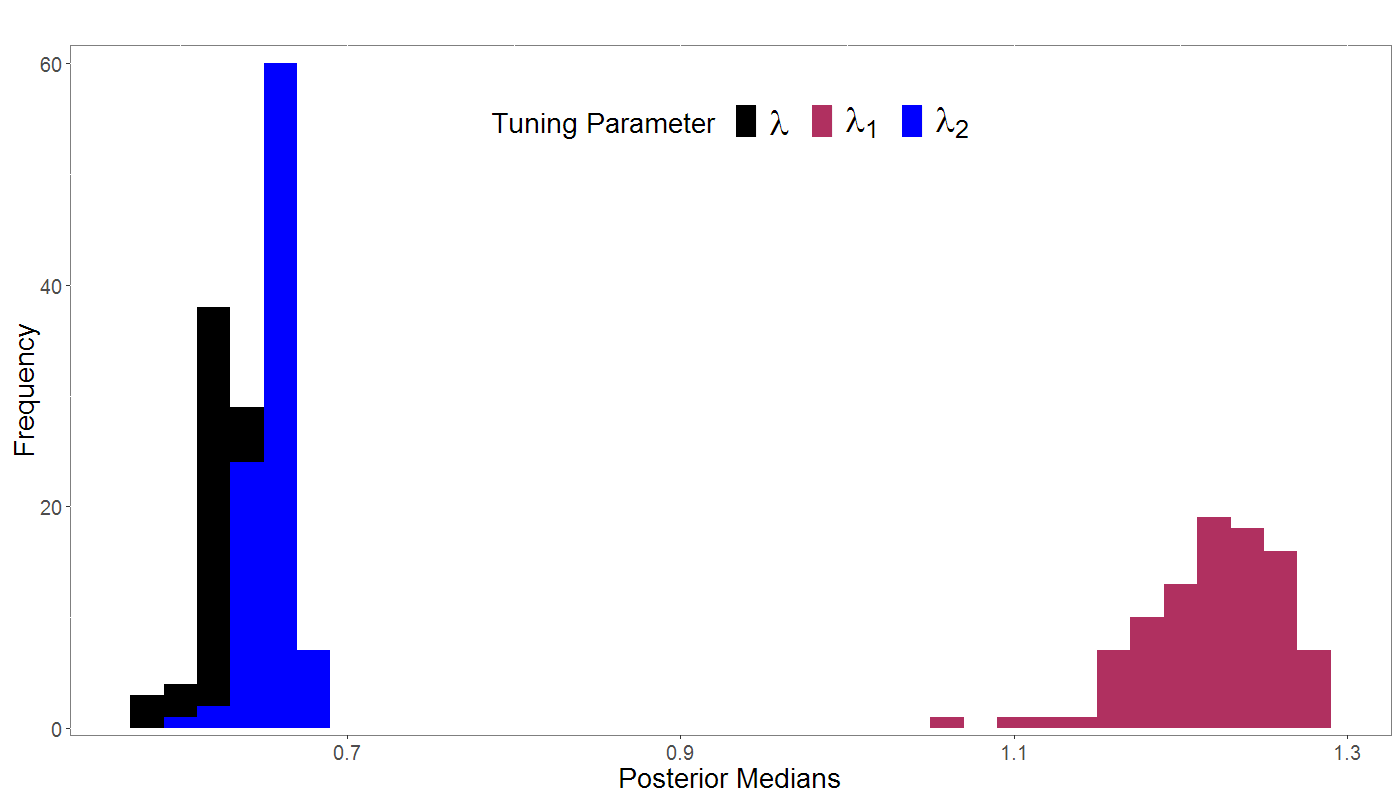
\includegraphics[scale=0.15]{rslambda}
\end{figure}
\end{itemize}

For BLASSO, 75\% of replications converged compared to 94\% for RS-BLASSO.

}

\frame{\frametitle{ Bayesian Shrinkage Estimation of LSTAR Models} 
\begin{itemize}
\item Bayesian Selection of the Threshold Variable\\~\

 Let $\bm{d}_t=[y_{t-1},y_{t-2},y_{t-3},y_{t-4}]'$ and $\bm{\phi}'=[\phi_1,\phi_2,\phi_3,\phi_4]$. 
Consider Reparameterized Model From Simulation 2 With Modified Threshold Variable $z_t=\bm{\phi}'\bm{d}_t$,
\begin{equation*}
	\begin{split}
		y_t&=(-0.6y_{t-3})[1-G(y_{t-1})]+(0.02+0.75y_{t-3})[G(y_{t-1})]+\epsilon_t\\
		& \textrm{where: } G(y_{t-1})=\bigg\{1+\exp\big[-120(\bm{\phi}'\bm{d}_t-0.02)\big]\bigg\}^{-1} \\
		&\textrm{ and }\epsilon_t \sim \textrm{i.i.d. }  N (0,0.02^2)\\
	\end{split}
\end{equation*}
Under  prior $\bm{\phi}\sim Dir([0.25,0.25,0.25,0.25]')$, we conduct posterior sampling for three different threshold variables $\{z_{1,t},z_{2,t},z_{3,t}\}$ defined through $\bm{\phi}$. BHS priors are used for autoregressive coefficients.
\end{itemize}
}

\frame{\frametitle{ Bayesian Shrinkage Estimation of LSTAR Models} 
\begin{itemize}
\item Bayesian Selection of the Threshold Variable (Scenario 1)\\~\

Consider Original Choice $z_{1,t}=y_{t-1}=[1,0,0,0]\bm{d}_t$. Posterior Means of $\bm{\phi}$ from 100 Replications are Plotted Below.
\begin{figure}[!h]
	\centering
      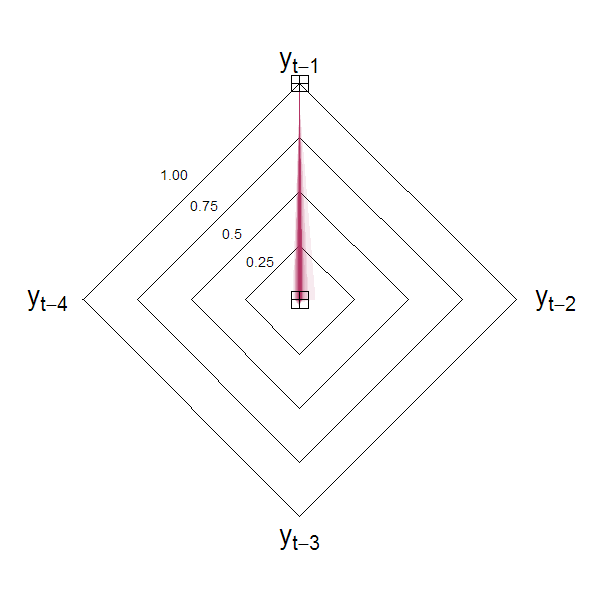
\includegraphics[scale=0.3]{hsthvar1}
\end{figure}
\end{itemize}
}

\frame{\frametitle{ Bayesian Shrinkage Estimation of LSTAR Models} 
\begin{itemize}
\item Bayesian Selection of the Threshold Variable (Scenario 2)\\~\

Consider  $z_{2,t}=y_{t-2}=[0,1,0,0]\bm{d}_t$. Posterior Means of $\bm{\phi}$ from 100 Replications are Plotted Below.
\begin{figure}[!h]
	\centering
      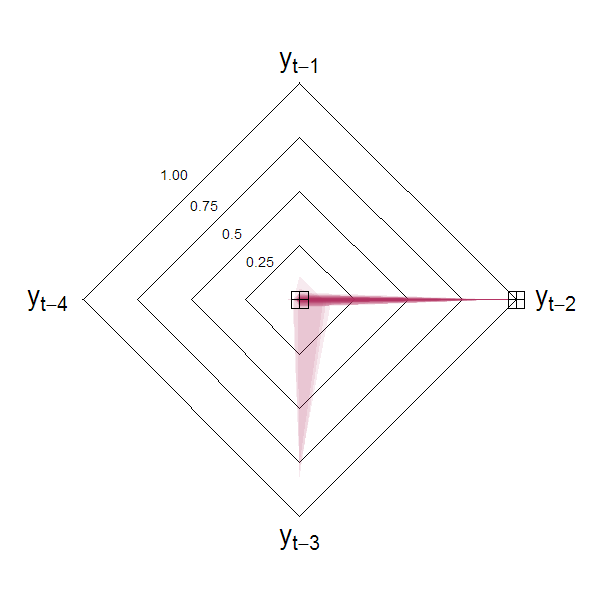
\includegraphics[scale=0.3]{hsthvar2}
\end{figure}
\end{itemize}
}

\frame{\frametitle{ Bayesian Shrinkage Estimation of LSTAR Models} 
\begin{itemize}
\item Bayesian Selection of the Threshold Variable (Scenario 3)\\~\

Consider  $z_{3,t}=\frac{y_{t-1}+y_{t-2}+y_{t-3}}{3}=[\frac{1}{3},\frac{1}{3},\frac{1}{3},0]\bm{d}_t$. Posterior Means of $\bm{\phi}$ from 100 Replications are Plotted Below.
\begin{figure}[!h]
	\centering
      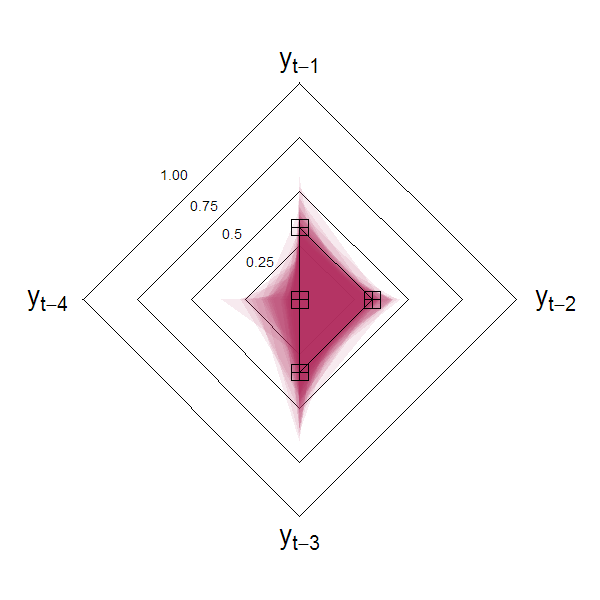
\includegraphics[scale=0.3]{hsthvar3}
\end{figure}
\end{itemize}
}

\frame{\frametitle{ Bayesian Shrinkage Estimation of LSTAR Models} 
\begin{itemize}
\item Application to Annual Sunspot Numbers\\~\
\begin{itemize}
	\item Textbook Example for Nonlinear Models Since \cite{Granger1957}
	\item Gathered and Updated by the World Data Center SILSO, Royal Observatory of Belgium, Brussels
	\item Square Root Transformation: $y_t=2[\sqrt{1+x_t}-1]$ \citep{Ghaddar1981}
	\item In \cite{Terasvirta2010}, LSTAR Outperformed Other AR, TAR,STAR, and Aritificial Neural Net (AR-NN) Models. Sparsity Achieved Via Stepwise Frequentist Procedure Using AIC
	\item Training Period (1700-1979) and Testing Period (1980-2006)
\end{itemize}
\end{itemize}
}

\frame{\frametitle{ Bayesian Shrinkage Estimation of LSTAR Models} 
\begin{itemize}
\item Application to Annual Sunspot Numbers (Cont.)\\~\
	\begin{itemize}
		\item Terasvirta's Best LSTAR Model ($F_T$)
		
		 	LSTAR(10) Model With $d=2$ \\~\
		\item Frequentist Estimation of Full Saturated LSTAR(10) ($F_S$)\\~\
		\item BHS Estimated Linear Model AR(10)  ($B_L$)\\~\
		\item BHS Estimated LSTAR(10) with $d=2$ ($B_2$)\\~\
		\item BHS Estimated LSTAR(10) Applying Dirichlet Prior ($B_D$)\\~\
		\item  BHS Estimated LSTAR(10)  with  $d=3$  ($B_3$)\\~\
	\end{itemize}
\end{itemize}
}

\frame{\frametitle{ Bayesian Shrinkage Estimation of LSTAR Models} 
\begin{itemize}
\item Application to Annual Sunspot Numbers (Cont.)\\~\

Compare Models on RMSFE($h$) for Horizons $h \in \{1,2,3,4,5\}$ \\~\

Bootstrap Method Used for Multi-step Ahead Forecasts for 1980-2006 \\~\

\begin{table}[!h]
  \centering
    \begin{tabular}{ccccccc}
    \toprule
     \multirow{2}[0]{*}{Model} & \multicolumn{5}{c}{Horizon} \\
                 & 1    & 2    & 3    & 4    & 5 \\
         \midrule
	\rowcolor{Gray}
     $F_T$ &  1.42 &  2    &  2.36 &  2.51 & 2.35 \\
            $F_S$ & 1.86 & 3.21 & 3.7  & 3.63 & 3.16 \\
         \midrule
       $B_L$ & 1.73 & 2.3  & 2.54 & 2.53 & 2.56 \\
	\rowcolor{Gray}
        $B_2$ & 1.42 & 1.96 &  2.29 &  2.19 & 2.19 \\
         $B_D$ & 1.77 & 2.83 & 3.38 & 3.5  & 3.29 \\
          $B_3$ & 1.86 & 3.11 & 3.58 & 3.62 & 3.58 \\
    \bottomrule
    \end{tabular}%
  \label{tab:ssrmsfe}%
\end{table}%
\end{itemize}
}

\frame{\frametitle{ Bayesian Shrinkage Estimation of LSTAR Models} 
\begin{itemize}
\item Application to Daily Maximum Water Temperatures\\~\
	\begin{itemize}
		\item Data Used From 31 Rivers in Spain
		\item Models Estimated to Forecast Daily Maximum Water Temperature Using Previously Known Daily Maximum Water Temperatures and Daily Maximum Air Temperatures
		\item Combination of BHS and Dirichlet Priors for Estimation of Linear and Nonlinear Models Under Assumption $P=6$
		\item Horizon Specific Models Targeting 3-step and 7-step Ahead Forecasts
		\item Nonlinear Models Improved Forecasting Accuracy for a Couple of Rivers (Details Provided in Paper) 
	\end{itemize}
\end{itemize}
}
%%%%%%%%%%%%%%%%%%%%%%%%%%%%%%%%%%%%%%%%%%%%%%









%%%%%%%%%%%%%%%%%%%%%%%%%%%%%%%%%%%%%%%%%%%%%%
\frame{\frametitle{Bayesian Model Selection of TAR Models} 
\begin{itemize}
	\item Consider General TAR($P$) Model
	
	\begin{equation*}
\begin{split}
y_t&=
  \begin{cases}
    \alpha_0+\alpha_1y_{t-1}+\alpha_2y_{t-2}+\cdots+\alpha_Py_{t-P}+\epsilon_{\alpha,t} & \textrm{ if } z_t<\delta \\
    \beta_0+\beta_1y_{t-1}+\beta_2y_{t-2}+\cdots+\beta_Py_{t-P}+\epsilon_{\beta,t} & \textrm{ if } z_t>\delta \\
  \end{cases}\\
  &=
    \begin{cases}
    \bm{\alpha}'\bm{y_{t-1}} +\epsilon_{\alpha,t} & \textrm{ if } z_t<\delta \\
     \bm{\beta}'\bm{y_{t-1}} +\epsilon_{\beta,t} & \textrm{ if } z_t>\delta \\
  \end{cases}\\
  \textrm{ where } & \epsilon_{\alpha,t} \sim N(0,\sigma^2_\alpha) \textrm{ and } \epsilon_{\beta,t} \sim N(0,\sigma^2_\beta)
  \end{split}
\end{equation*}
	
	For future reference, we abbreviate the full TAR($P$) model $\mathcal{M}_R$. \\~\
	
	Model $\mathcal{M}_R$ is fully defined by parameter vector $\bm{\theta}_{\mathcal{M}_R}'=[\bm{\alpha}',\bm{\beta}',\sigma_\alpha,\sigma_\beta,\delta]$. \\~\
	
	Furthermore, let $\mathcal{M}_{LR}$ and $\mathcal{M}_{HR}$ represent the low-regime and high-regime models, respectively.\\~\
	

From the $2^{2(P+1)}$ submodels, we aim to identify the best submodel $\mathcal{M}^*_R$
\end{itemize}
}

\frame{\frametitle{Bayesian Model Selection of TAR Models} 
\begin{itemize}
\item Methodology Step 1: Bayesian Shrinkage\\~\

Apply Regime-Specific BHS for Initial Sparse Estimation
\begin{equation*}
\label{eq:hsp}
\begin{split}
 	\alpha_j &\sim N(0,\sigma^2_\alpha\lambda^2_{\alpha_j}\lambda_{\alpha}^2), \textrm{ } \lambda_{\alpha_j}\sim C^+(0,1), \textrm{ } \lambda_\alpha \sim C^+(0,1) \\
 	\beta_j & \sim N(0,\sigma^2_\beta\lambda^2_{\beta_j}\lambda_{\beta}^2), \textrm{ } \lambda_{\beta_j}\sim C^+(0,1), \textrm{ } \lambda_\beta \sim C^+(0,1)\\
 	& \forall j \in \{1,2,3,\cdots,P\}
\end{split}
\end{equation*}

\end{itemize}
}

\frame{\frametitle{Bayesian Model Selection of TAR Models} 
\begin{itemize}
	\item Methodology Step 2: Projection Predictive Variable Selection\\~\
	\begin{itemize}
		\item Kullback-Leibler (KL) Divergence
		\begin{itemize}
			\item Asymmetric Measure of Distance Between 2 Probability Distributions
			\item Developed by \cite{Goutis1998, Dupuis2003,Piironen2017} for Generalized Linear Models
			\item Measure Discrepancy Between Full Model $\mathcal{M}_R$ and Proposed Submodel $\mathcal{M}^\perp_R$ \\~\
		\end{itemize}
		\item Necessary Definitions
			$$\textrm{Matrix } \bm{Y_{t-1}} \textrm{ where $k$th row is } \bm{y_{k-1}}'=[1,y_{k-1},y_{k-2},\cdots,y_{k-P}]$$
			$$\textrm{Regime-Specific Full Reference Models: } \mathcal{M}_{LR} \textrm{ and } \mathcal{M}_{HR}$$
			$$\textrm{Regime-Specific Submodels: } \mathcal{M}^\perp_{LR} \textrm{ and } \mathcal{M}^\perp_{HR}$$
	\end{itemize}
\end{itemize}
}

\frame{\frametitle{Bayesian Model Selection of TAR Models} 
\begin{itemize}
	\item Methodology Step 2: Projection Predictive Variable Selection (Cont.)\\~\
	 \begin{itemize}
		\item Regime-Specific Projection Approach\\~\
		\begin{equation*}
		\begin{split}
		f(\bm{\theta}_{\mathcal{M}_R}|\mathcal{M}_R,Data) & \to f(\bm{\theta}_{\mathcal{M}^\perp_R}|\mathcal{M}^\perp_R,Data)\\
		\bm{\theta}^{(s)} & \to \bm{\theta}^{\perp(s)}\\
		[\bm{\alpha}^{(s)},\sigma_\alpha^{(s)},\bm{\beta}^{},\sigma_\beta^{(s)},\delta^{(s)}] & \to [\bm{\alpha}^{\perp(s)},\sigma_\alpha^{\perp(s)},\bm{\beta}^{\perp(s)},\sigma_\beta^{\perp(s)},\delta^{(s)}]\\
		\end{split}
		\end{equation*}
		\item Regime-Specific Projection Process

\indent Split $\bm{Y_{t-1}}$ into $\bm{Y_{LR,t-1}}$ and $\bm{Y_{HR,t-1}}$ based on $\delta^{(s)}$.

\indent Identify $\bm{Y^\perp_{LR,t-1}}$ and $\bm{Y^\perp_{HR,t-1}}$ based on proposed  $\mathcal{M}^\perp_{LR}$ and $\mathcal{M}^\perp_{HR}$

\begin{equation*}
\scriptsize
\begin{split}
\bm{\alpha}^{\perp(s)}&=(\bm{Y^{\perp'}_{LR,t-1}}\bm{Y^{\perp}_{LR,t-1}})^{-1} \bm{Y^{\perp'}_{LR,t-1}}     \bm{Y_{LR,t-1}}\bm{\alpha}^{(s)}\\
\sigma_\alpha^{\perp(s)}&=\sqrt{\sigma_\alpha^{(s)}+\frac{( \bm{Y_{LR,t-1}}\bm{\alpha}^{(s)}-\bm{Y^\perp_{LR,t-1}}\bm{\alpha}^{\perp(s)})'( \bm{Y_{LR,t-1}}\bm{\alpha}^{(s)}-\bm{Y^\perp_{LR,t-1}}\bm{\alpha}^{\perp(s)})}{T}                                  }\\
\bm{\beta}^{\perp(s)}&=(\bm{Y^{\perp'}_{HR,t-1}}\bm{Y^{\perp}_{HR,t-1}})^{-1} \bm{Y^{\perp'}_{HR,t-1}} \bm{Y_{HR,t-1}}\bm{\beta}^{(s)}\\
\sigma_\beta^{\perp(s)}&=\sqrt{\sigma_\beta^{(s)}+\frac{( \bm{Y_{HR,t-1}}\bm{\beta}^{(s)}-\bm{Y^\perp_{HR,t-1}}\bm{\beta}^{\perp(s)})'( \bm{Y_{HR,t-1}}\bm{\beta}^{(s)}-\bm{Y^\perp_{HR,t-1}}\bm{\beta}^{\perp(s)})}{T}                                   }
\end{split}
\end{equation*}
	\end{itemize}
\end{itemize}
}

\frame{\frametitle{Bayesian Model Selection of TAR Models} 
\begin{itemize}
	\item Methodology Step 2: Projection Predictive Variable Selection (Cont.)\\~\
	 \begin{itemize}
		\item Regime-Specific Projection Process (Cont.)\\~\
		For each $\bm{\theta}^{(s)}$, we obtain regime-specific KL divergences,
\begin{equation*}
\begin{split}
d^{(s)}_{LR}(\bm{\alpha}^{(s)},\sigma^{(s)}_\alpha)&=\frac{1}{2}\log\bigg(\frac{\sigma^{\perp(s)}_\alpha}{\sigma^{(s)}_\alpha}\bigg)\\
d^{(s)}_{HR}(\bm{\beta}^{(s)},\sigma^{(s)}_\beta)&=\frac{1}{2}\log\bigg(\frac{\sigma^{\perp(s)}_\beta}{\sigma^{(s)}_\beta}\bigg)
\end{split}
\end{equation*}
	
		Finally, we measure regime-specific discrepancies by
\begin{equation*}
\begin{split}
D(\mathcal{M}_{LR}||\mathcal{M}^\perp_{LR})&=\frac{1}{S}\sum\limits^S_{s=1} d^{(s)}_{LR}(\bm{\alpha}^{(s)},\sigma^{(s)}_\alpha)    \\
D(\mathcal{M}_{HR}||\mathcal{M}^\perp_{HR})&=\frac{1}{S}\sum\limits^S_{s=1} d^{(s)}_{HR}(\bm{\beta}^{(s)},\sigma^{(s)}_\beta)     \\
\end{split}
\end{equation*}
	\end{itemize}
\end{itemize}
}

\frame{\frametitle{Bayesian Model Selection of TAR Models} 
\begin{itemize}
	\item Methodology Step 2: Projection Predictive Variable Selection (Cont.)\\~\
	 \begin{itemize}
		\item Forward Stepwise Selection Algorithm\\~\
		
		For Intercept-only Models $\mathcal{M}^0_{LR}$ and $\mathcal{M}^0_{HR}$, calculate initial discrepancies $D(\mathcal{M}_{LR}||\mathcal{M}^0_{LR})$ and $D(\mathcal{M}_{HR}||\mathcal{M}^0_{HR})$	\\~\
	
		For each level of flexibility $p \in \{1,2,\cdots,P\}$, we identify the best regime-specific submodels $\mathcal{M}^p_{LR}$ and $\mathcal{M}^p_{HR}$.\\~\
		
		Algorithm conducted such that for $j<k$ $\mathcal{M}^j_{HR}$ is nested in $\mathcal{M}^k_{HR}$.
	\end{itemize}
\end{itemize}
}

\frame{\frametitle{Bayesian Model Selection of TAR Models} 
\begin{itemize}
	\item Methodology Step 3: Final Model Selection\\~\
	 \begin{itemize}
		\item Choose $\mathcal{M}^*_{LR}$ and $\mathcal{M}^*_{HR}$ Based on Relative Explanatory Power \\~\
		\begin{equation*}
\begin{split}
RelE(\mathcal{M}^p)&=1-\frac{D(\mathcal{M}||\mathcal{M}^p)}{D(\mathcal{M}||\mathcal{M}^0)}\\
\end{split}
\end{equation*}
		\item Choose Based On Minimization of RMSFE for Time Period Intentionally Ignored
		\begin{equation*}
  			RMSFE(\mathcal{M}^p)=\sqrt{\frac{1}{T}\sum (y_t-\hat{y}_t)^2}
		\end{equation*}
	\end{itemize}
\end{itemize}
}

%%%%%%%%%%%%%%%%%%%%%%%%%%%%%%%%%%%%%%%%%%%%%%


\frame[plain,c] {\frametitle{Conclusion}
\begin{center}
{\Huge  Current Work} \\

\bigskip \bigskip

Autoregressive Moving Average Model: ARMA($p$,$q$)
\end{center}
\begin{equation*}
\bigg(1-\sum\limits_{i=1}^{p}\phi_{i}B^i\bigg)y_{t}=\bigg(1+\sum\limits_{j=1}^{q}\theta_{j}B^j\bigg)\epsilon_{t}
\end{equation*}

\begin{center}
We utilize the backshift operator $B$ where $B^ky_{t}=y_{t-k}$,\\ and assume $\epsilon_t\sim N(0,\sigma^2)$
\end{center}
}

\frame[plain,c] {\frametitle{Conclusion}
\begin{center}
{\Huge Questions}
\end{center}
}

























\frame[allowframebreaks]{\frametitle{References}
    {\footnotesize
    \bibliographystyle{apalike}
    \bibliography{phd}
    }
}

\end{document}

